\documentclass[12pt]{article}
\usepackage{graphicx}
\usepackage{caption}
\usepackage{subcaption}
%
% Title[Enter title of the experiment here]
\title{EE236: Experiment No. 1\\
RC Circuits}

% Author[Enter details of author here]
\author{Mohd Safwan, 17D070047}

% begin the document.
\begin{document}

% make a title page.[this creates title page]
\maketitle

\textbf{ ** All experiment reports may not contain all fields in this format,This document is just for your reference**} 

\section{Overview of the experiment} %[This segment creates Section as seen in document]

\subsection{Aim of the experiment}%[This segment creates sebsections under the same section]

To measure voltage across capacitor aginst square wave voltage of different frequecies.

\subsection{Methods}




In your own words, describe how you set out to realize the goal of the experiment. Only 1 paragraph of a brief overview of your approach is expected here. Do not list your observations here.
I used 

\section{Design}%[To add multiple sections, keep appending blocks like this]

In this section, explain your design strategy for the experiment.Mention all the design steps you follow for each part of the experiment.An equation based analysis, with supporting circuit diagrams is expected. Circuit diagrams must be made in Xcircuit.
 
 \begin{equation}
     v_{o1}-v_{o2}
     \newline
     = -g_mR_D(v_{in1}-v_{in2})
 \end{equation}     
 
 \begin{equation}
     a=b+c
 \end{equation}     

 %equations are to inserted in this manner.


\textbf{(copy-paste from handout will be counted as plagiarism).} 

%\textbf{this command prints text inside it in bold style}


\section{Simulation results}%[One more section]
\subsection{Code snippet}

Enter your ngspice code here:

*IV Charactersics of Normal Diode\\
* Resistive Load\\
R1 1 2 100\\
* Default Diode\\
D1 3 0 \\
*Dummy voltage source to measure current.\\
v1 2 3 dc 0v\\
* Voltage Source\\
Vin 1 0 dc 5.0v\\
* DC analysis: Vin is swept from 0.0V to 6.0V in steps of 0.05V\\
.control \\
dc Vin 0.0001 6 0.0001\\
run\\
* white background\\
set color0 =white\\
set color1=black\\
plot i(v1) vs V(2) \\
.endc\\
.end\\



\newpage
\subsection{Simulation results}

	Enter your simulation plots, together with text explaining the plots. All figures must have legible fonts, and a caption that makes sense.
 \begin{figure}[h]
 \centering
 \begin{subfigure}{.5\textwidth}
   \centering
   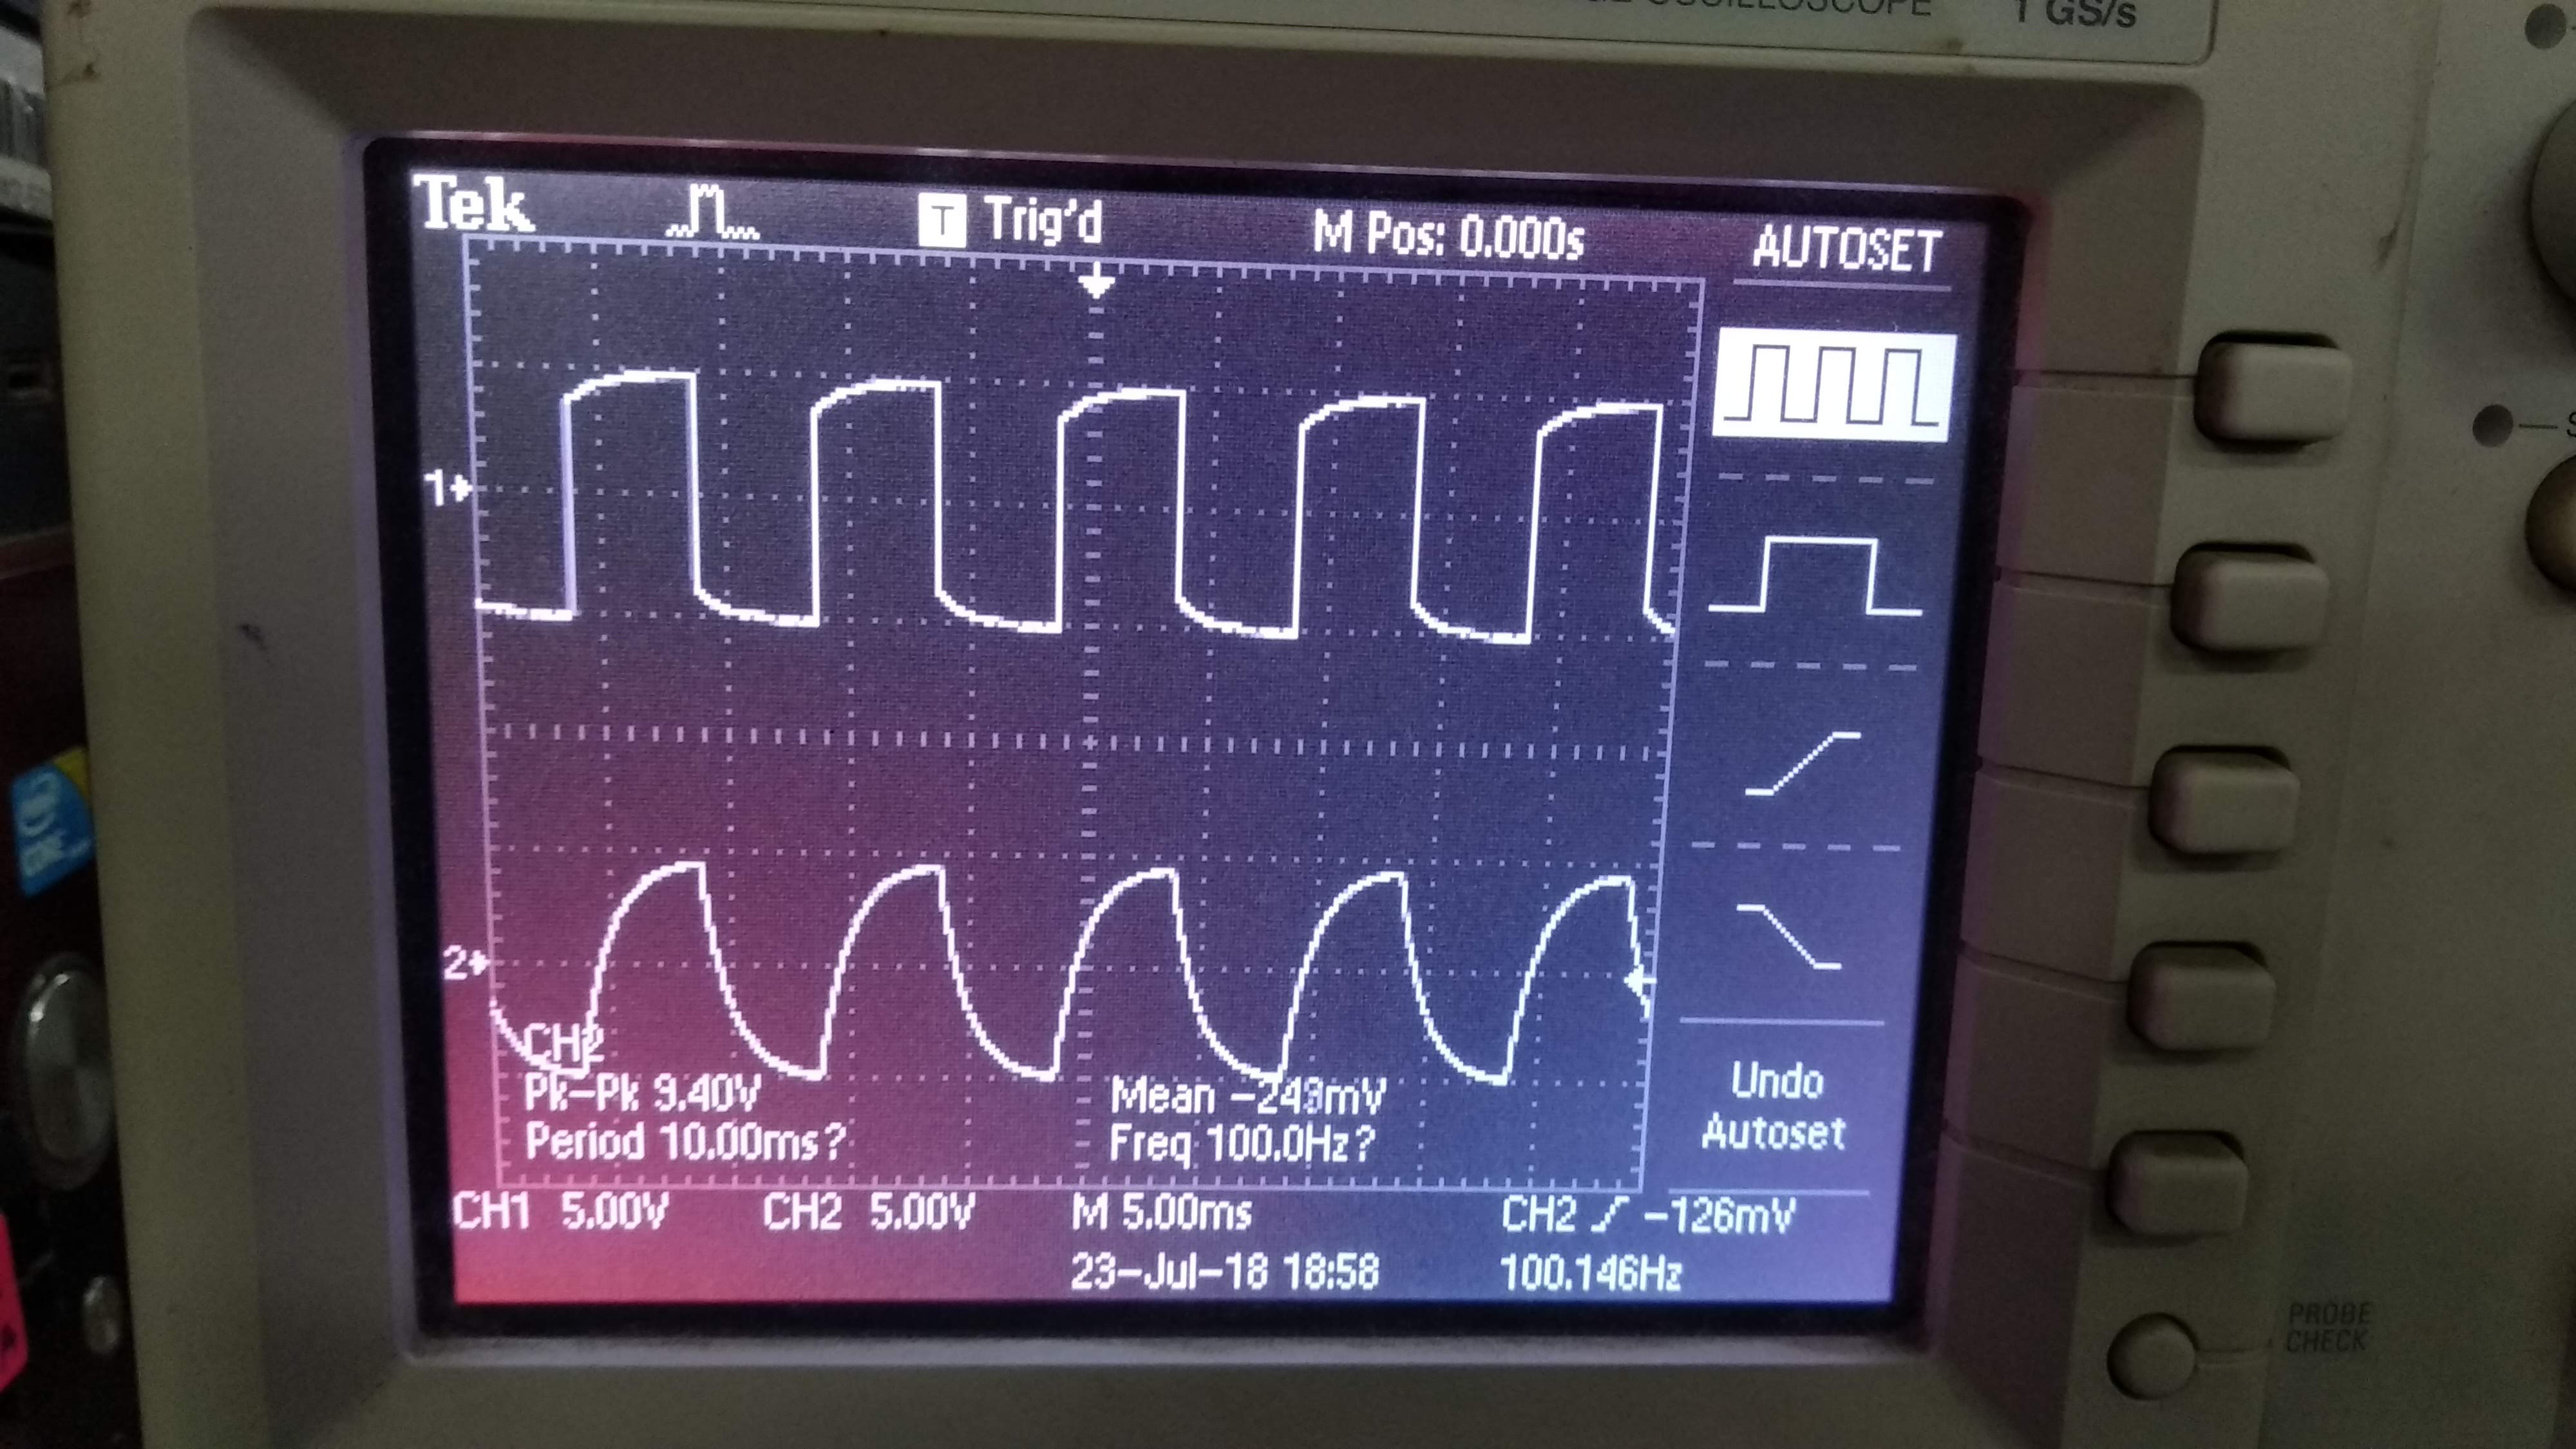
\includegraphics[scale=0.045]{100hz.jpg}
   \caption{100Hz}
   \label{fig:sub1}
 \end{subfigure}%
 \begin{subfigure}{.5\textwidth}
   \centering
   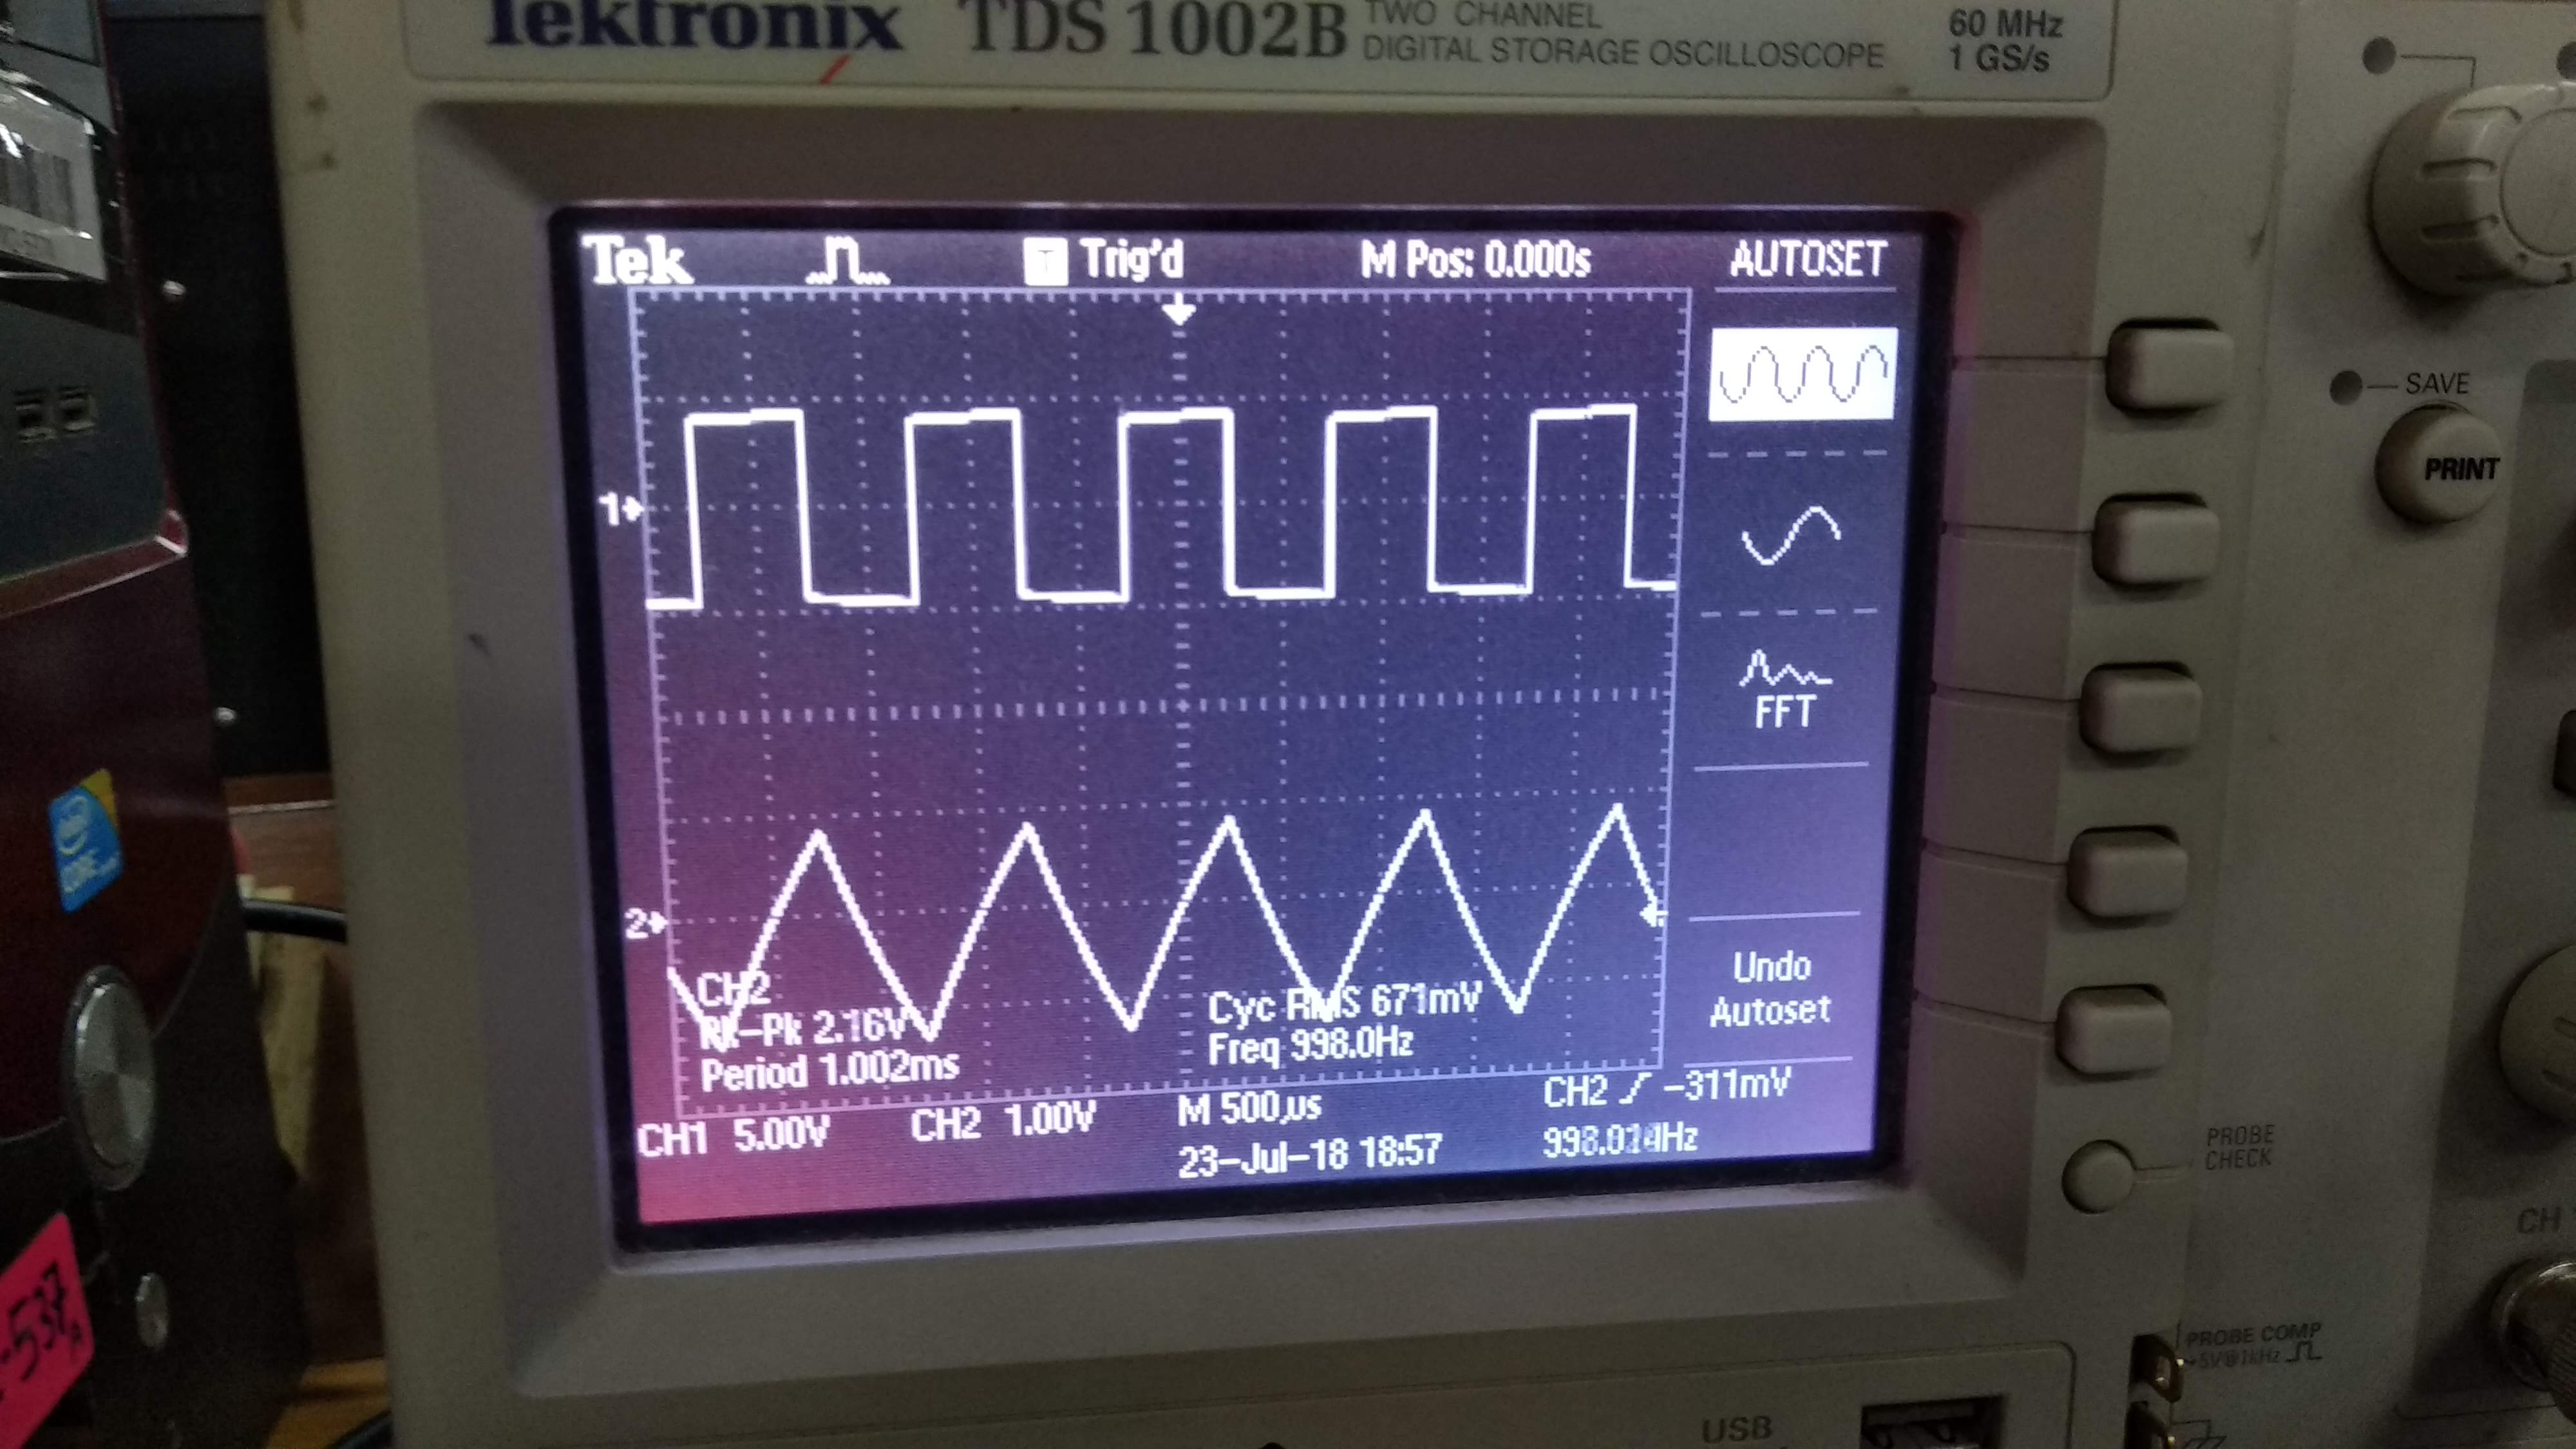
\includegraphics[scale=0.045]{1000hz.jpg}
   \caption{1000Hz}
   \label{fig:sub2}
 \end{subfigure}
 \label{fig:test}
 \end{figure}

 \begin{figure}[h]
 \centering
 \begin{subfigure}{.5\textwidth}
   \centering
   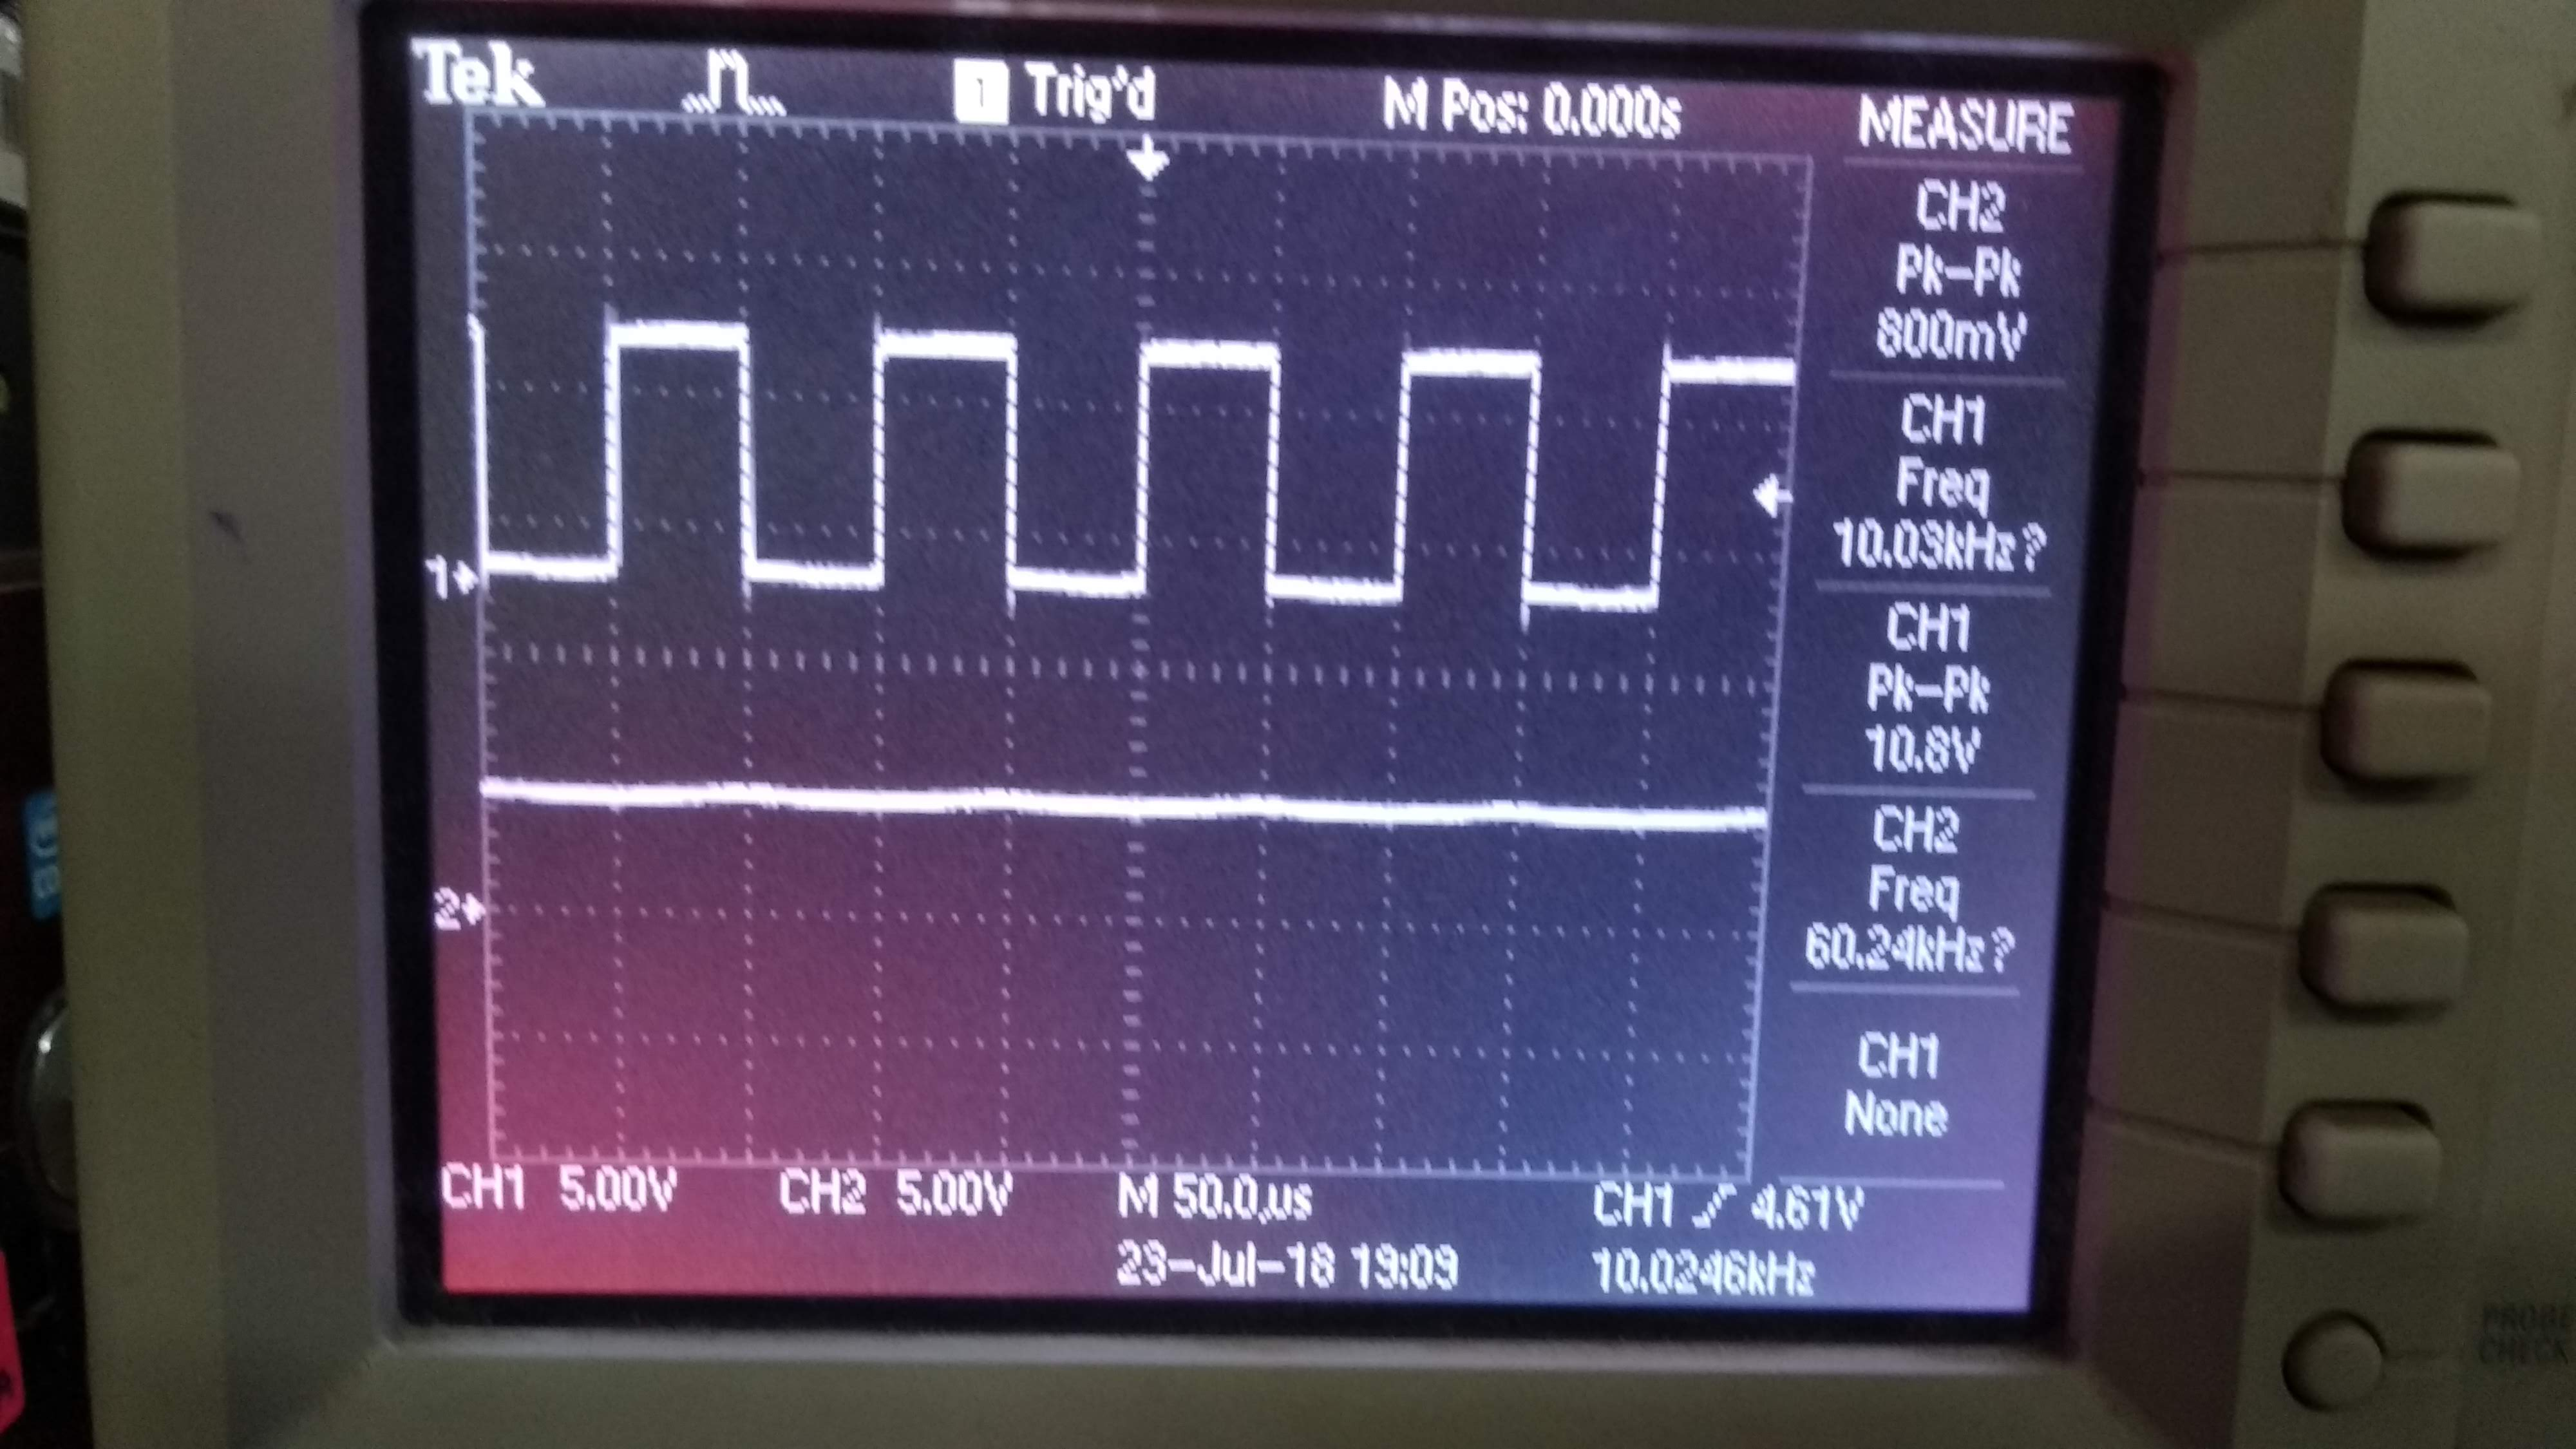
\includegraphics[scale=0.045]{10khz.jpg}
   \caption{10kHz}
   \label{fig:test1}
 \end{subfigure}%
 \begin{subfigure}{.5\textwidth}
   \centering
   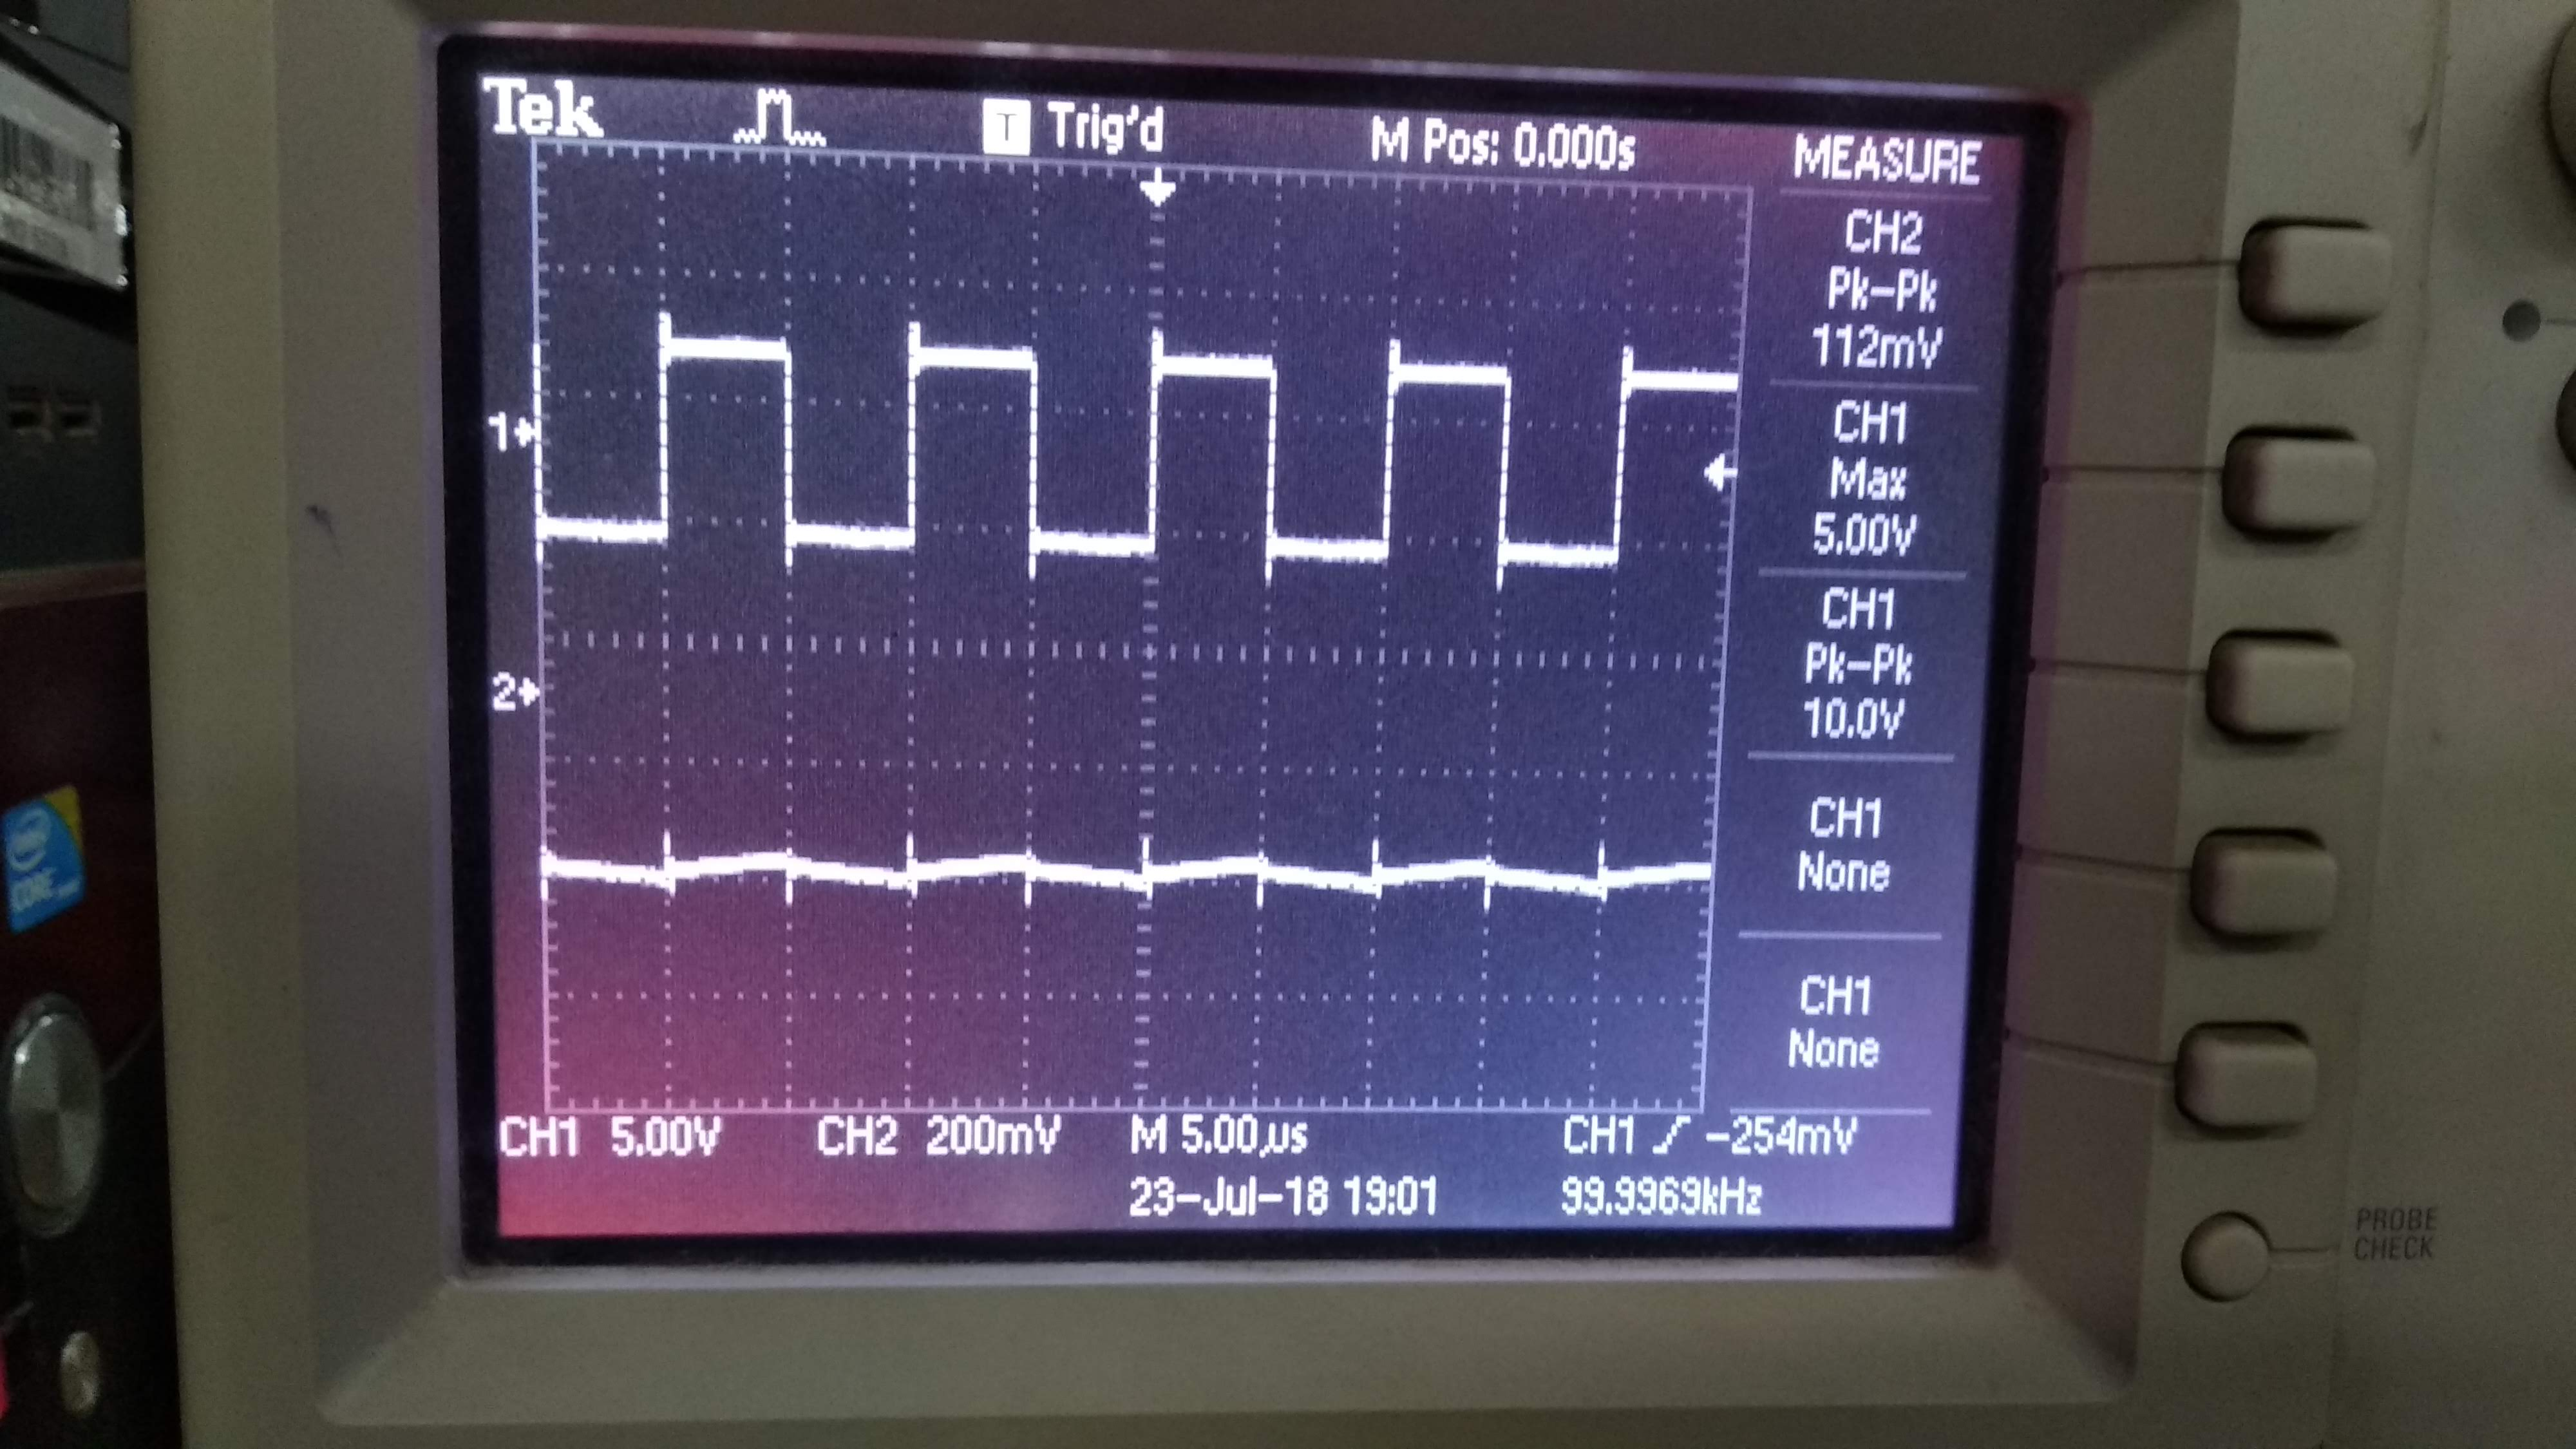
\includegraphics[scale=0.045]{100khz.jpg}
   \caption{100kHz}
   \label{fig:test2}
 \end{subfigure}
 \end{figure}




\section{Experimental results}

\subsection{Part-1}

Results of part 1 of experiment should be added here.Mention what component values you used with appropriate circuit diagram, and what your measured values were.

\begin{table}[!hbt]
		% Center the table
		\begin{center}
		\caption{Table Caption}
		\begin{tabular}{|c|c|c|c|}
			% To create a horizontal line, type \hline
			\hline
			% To end a column type &
			% For a linebreak type \\
			Sr. No. & column1 & column2 & column3\\
			\hline
			row1 &  &  & \\
			\hline
			row2 &  &  & \\
			\hline
            
		\end{tabular}
		\end{center}
\end{table}

\subsection{Part-2}

Mention what component values you used with appropriate circuit diagram, and what your measuSred values were. Add any DSO screen captures you may have got on your phone. Address all the questions which are asked in the labsheet.\

\subsection{Part-3}

Mention what component values you used with appropriate circuit diagram, and what your measured values were. Add any DSO screen captures you may have got on your phone. Address all the questions asked in labsheet and try to write explanations for the results you obtain.

\begin{figure}
\centering
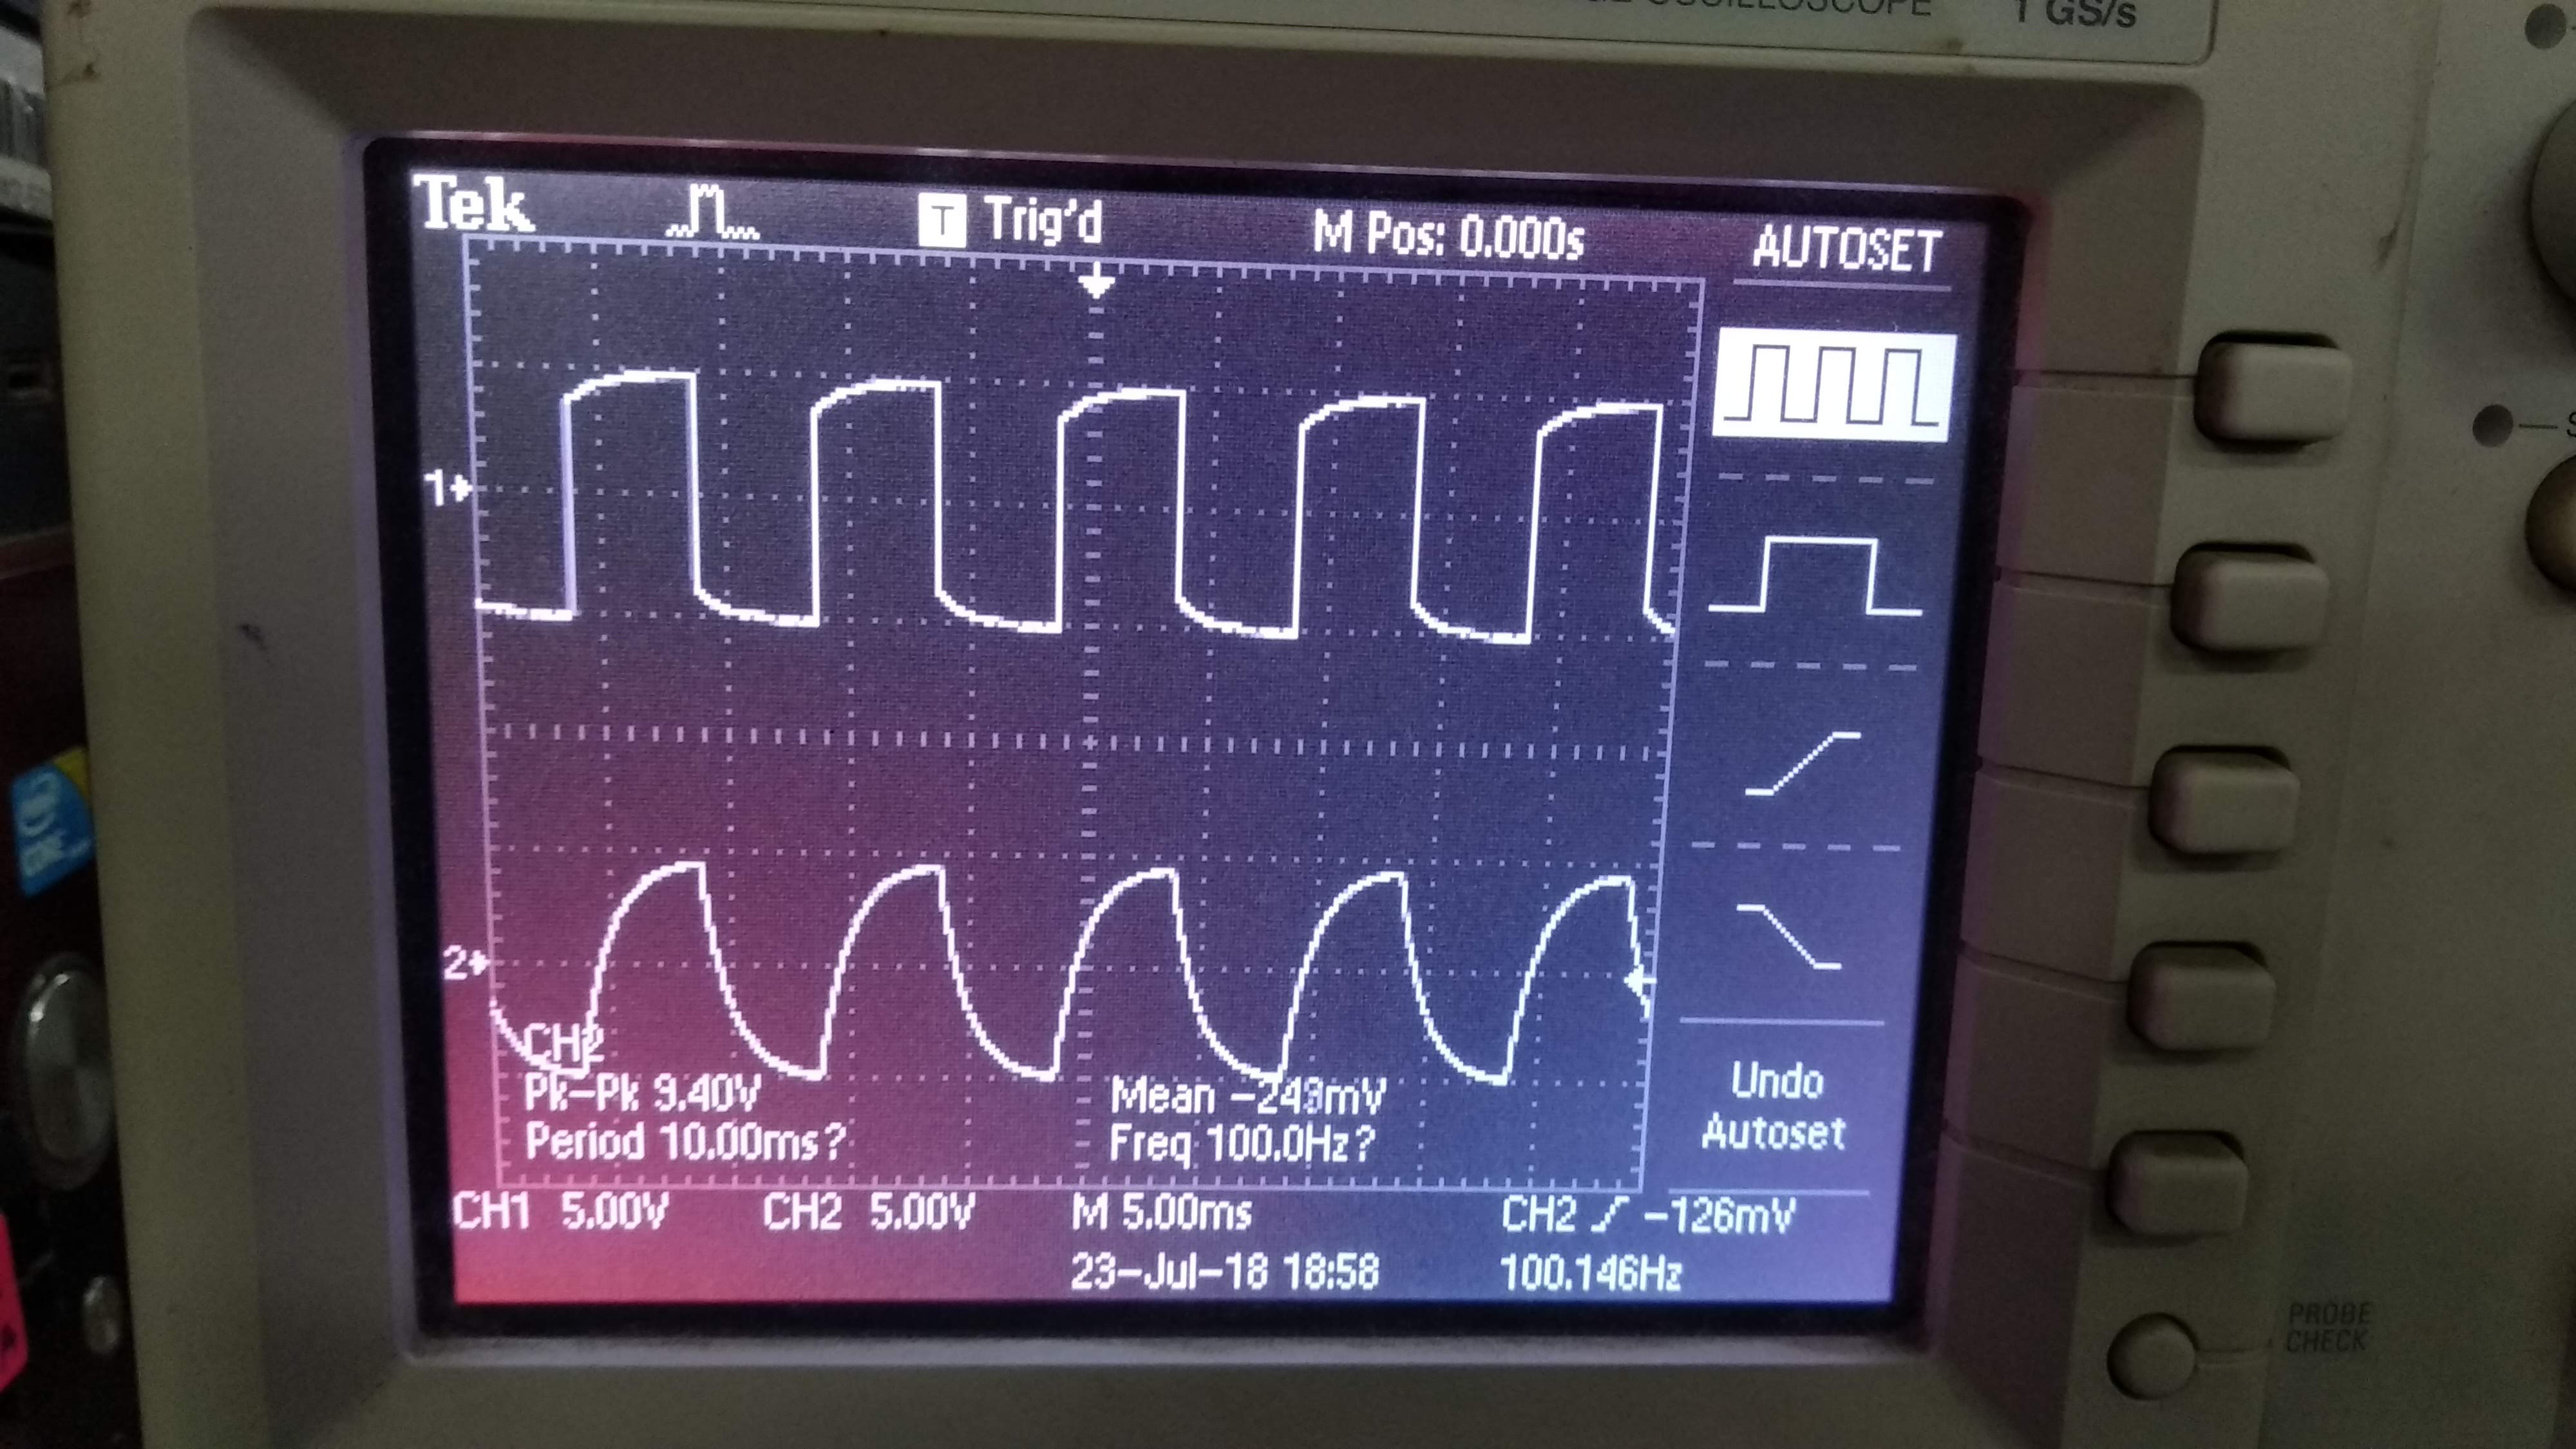
\includegraphics[scale = 0.08]{100hz.jpg}
\end{figure}

\begin{figure}
\centering
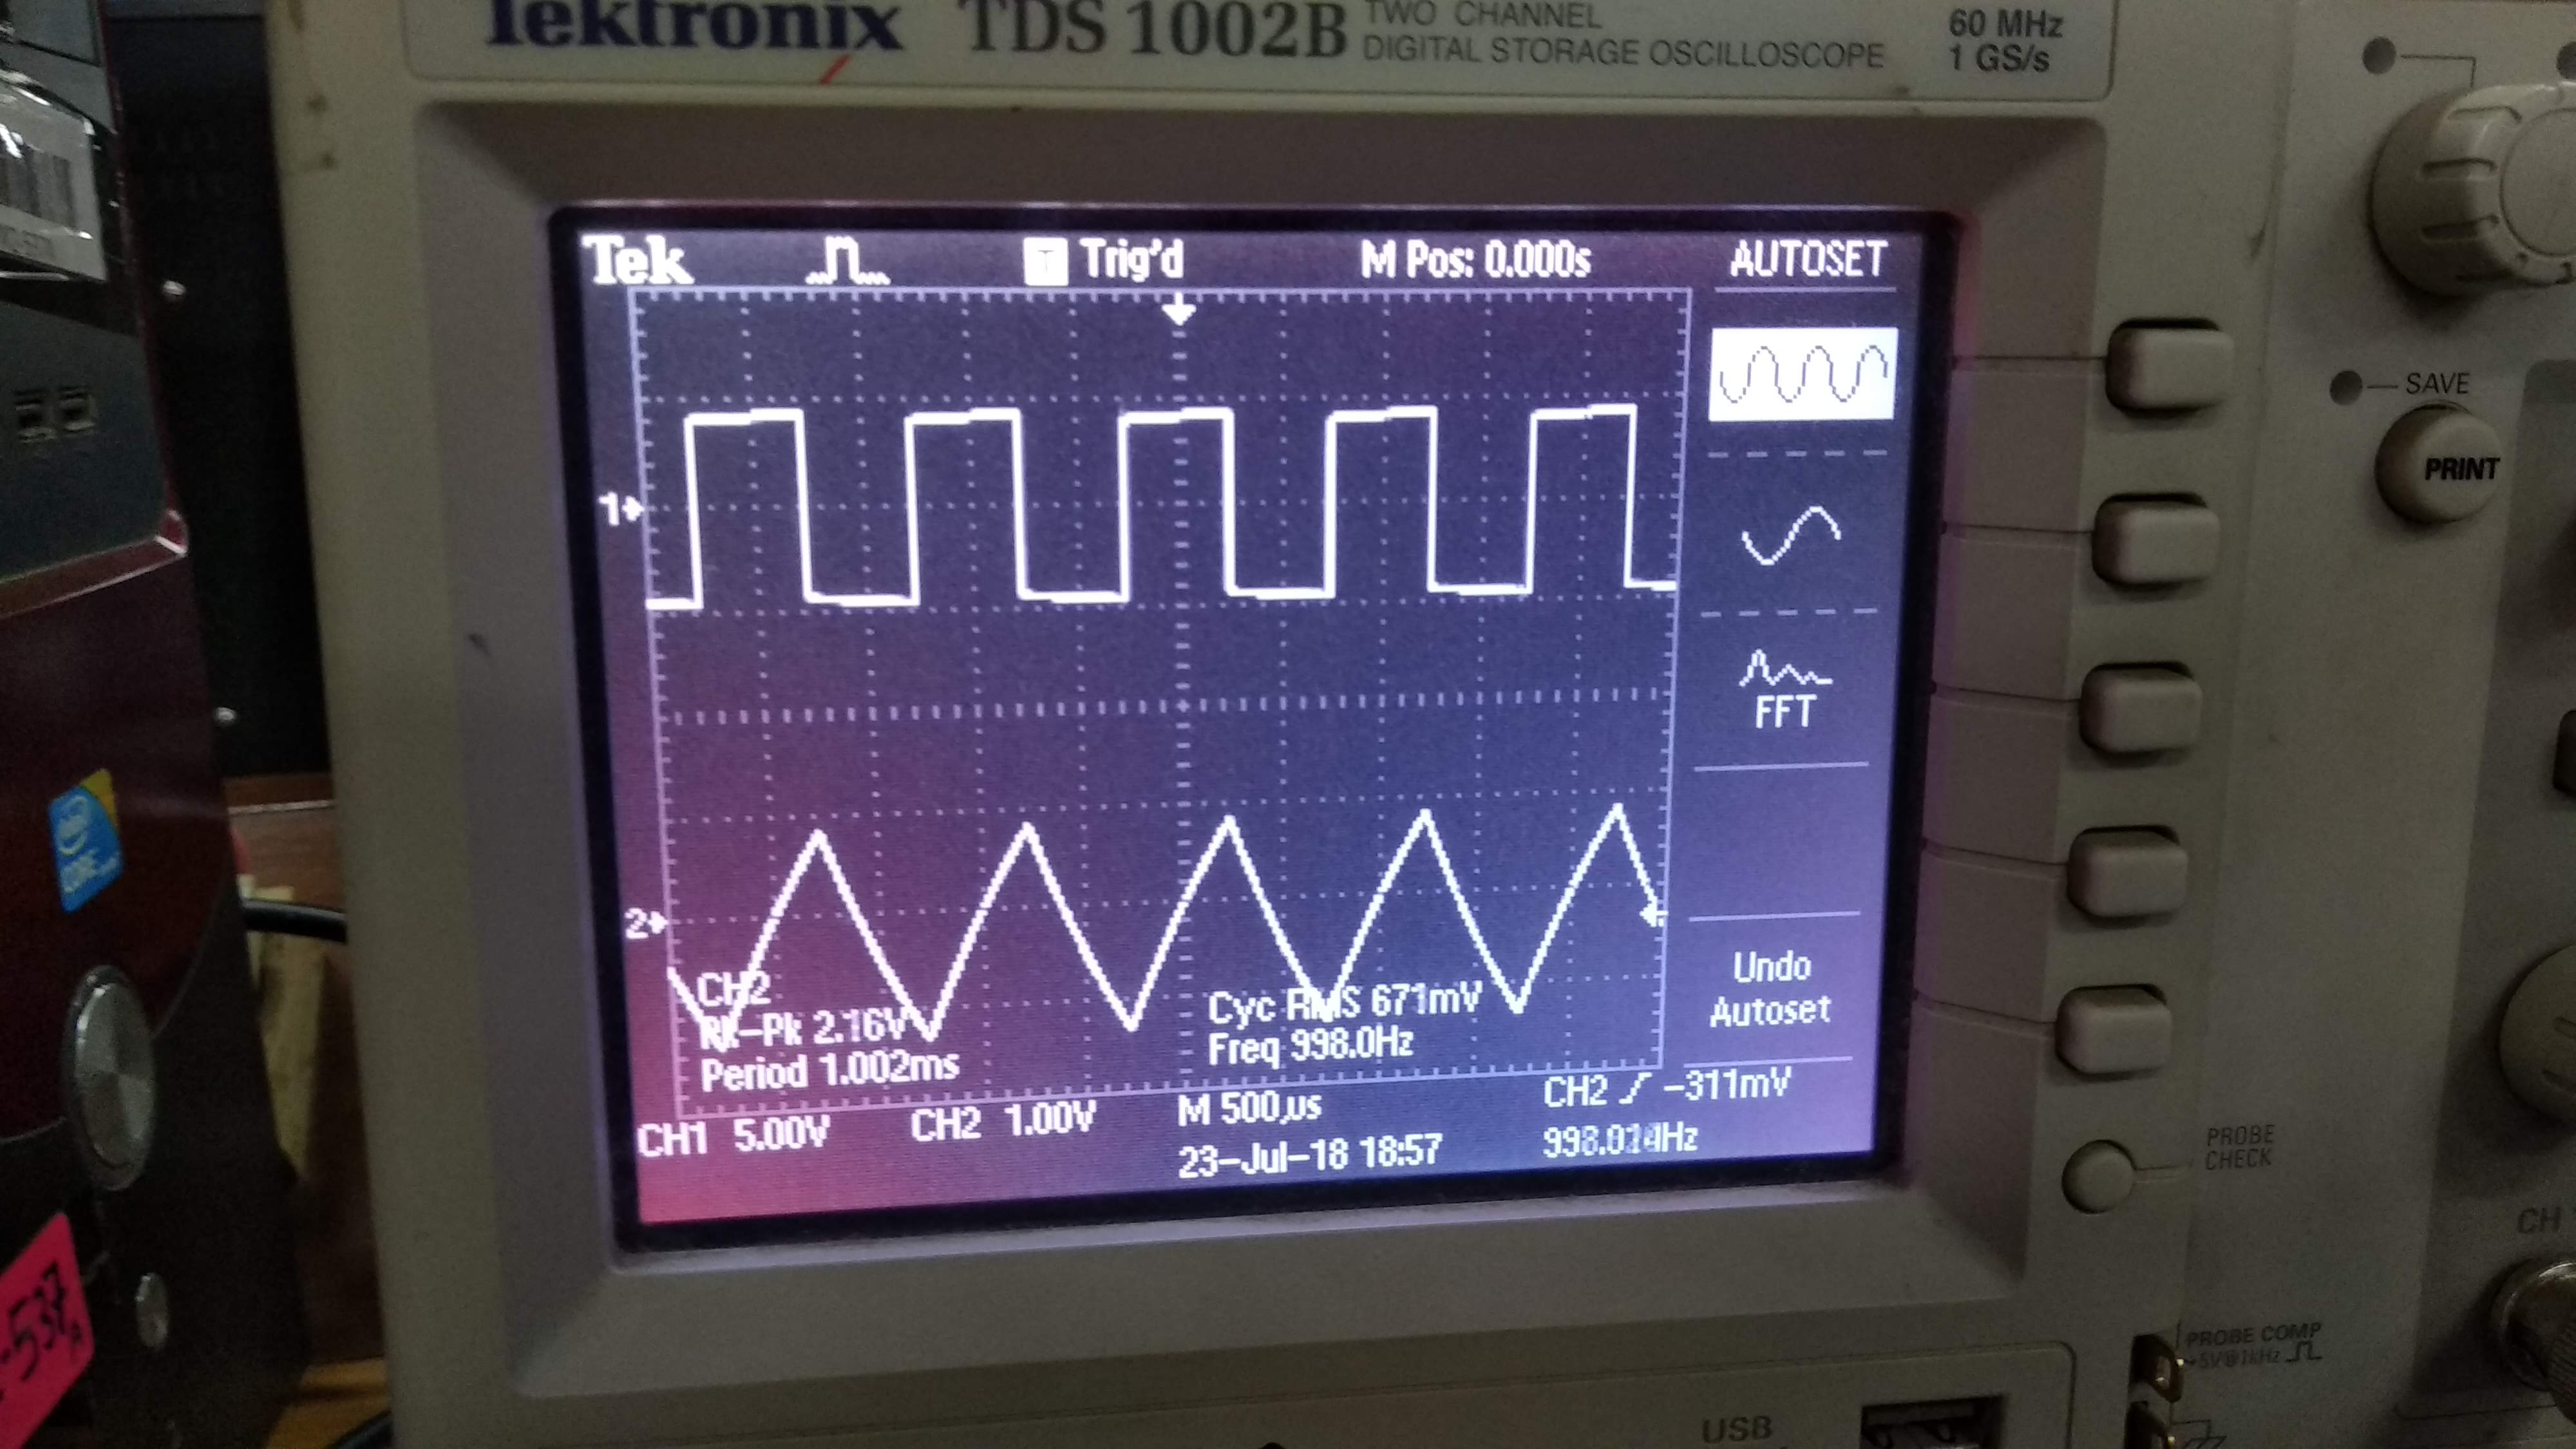
\includegraphics[scale = 0.08]{1000hz.jpg}
\end{figure}

\begin{figure}
\centering
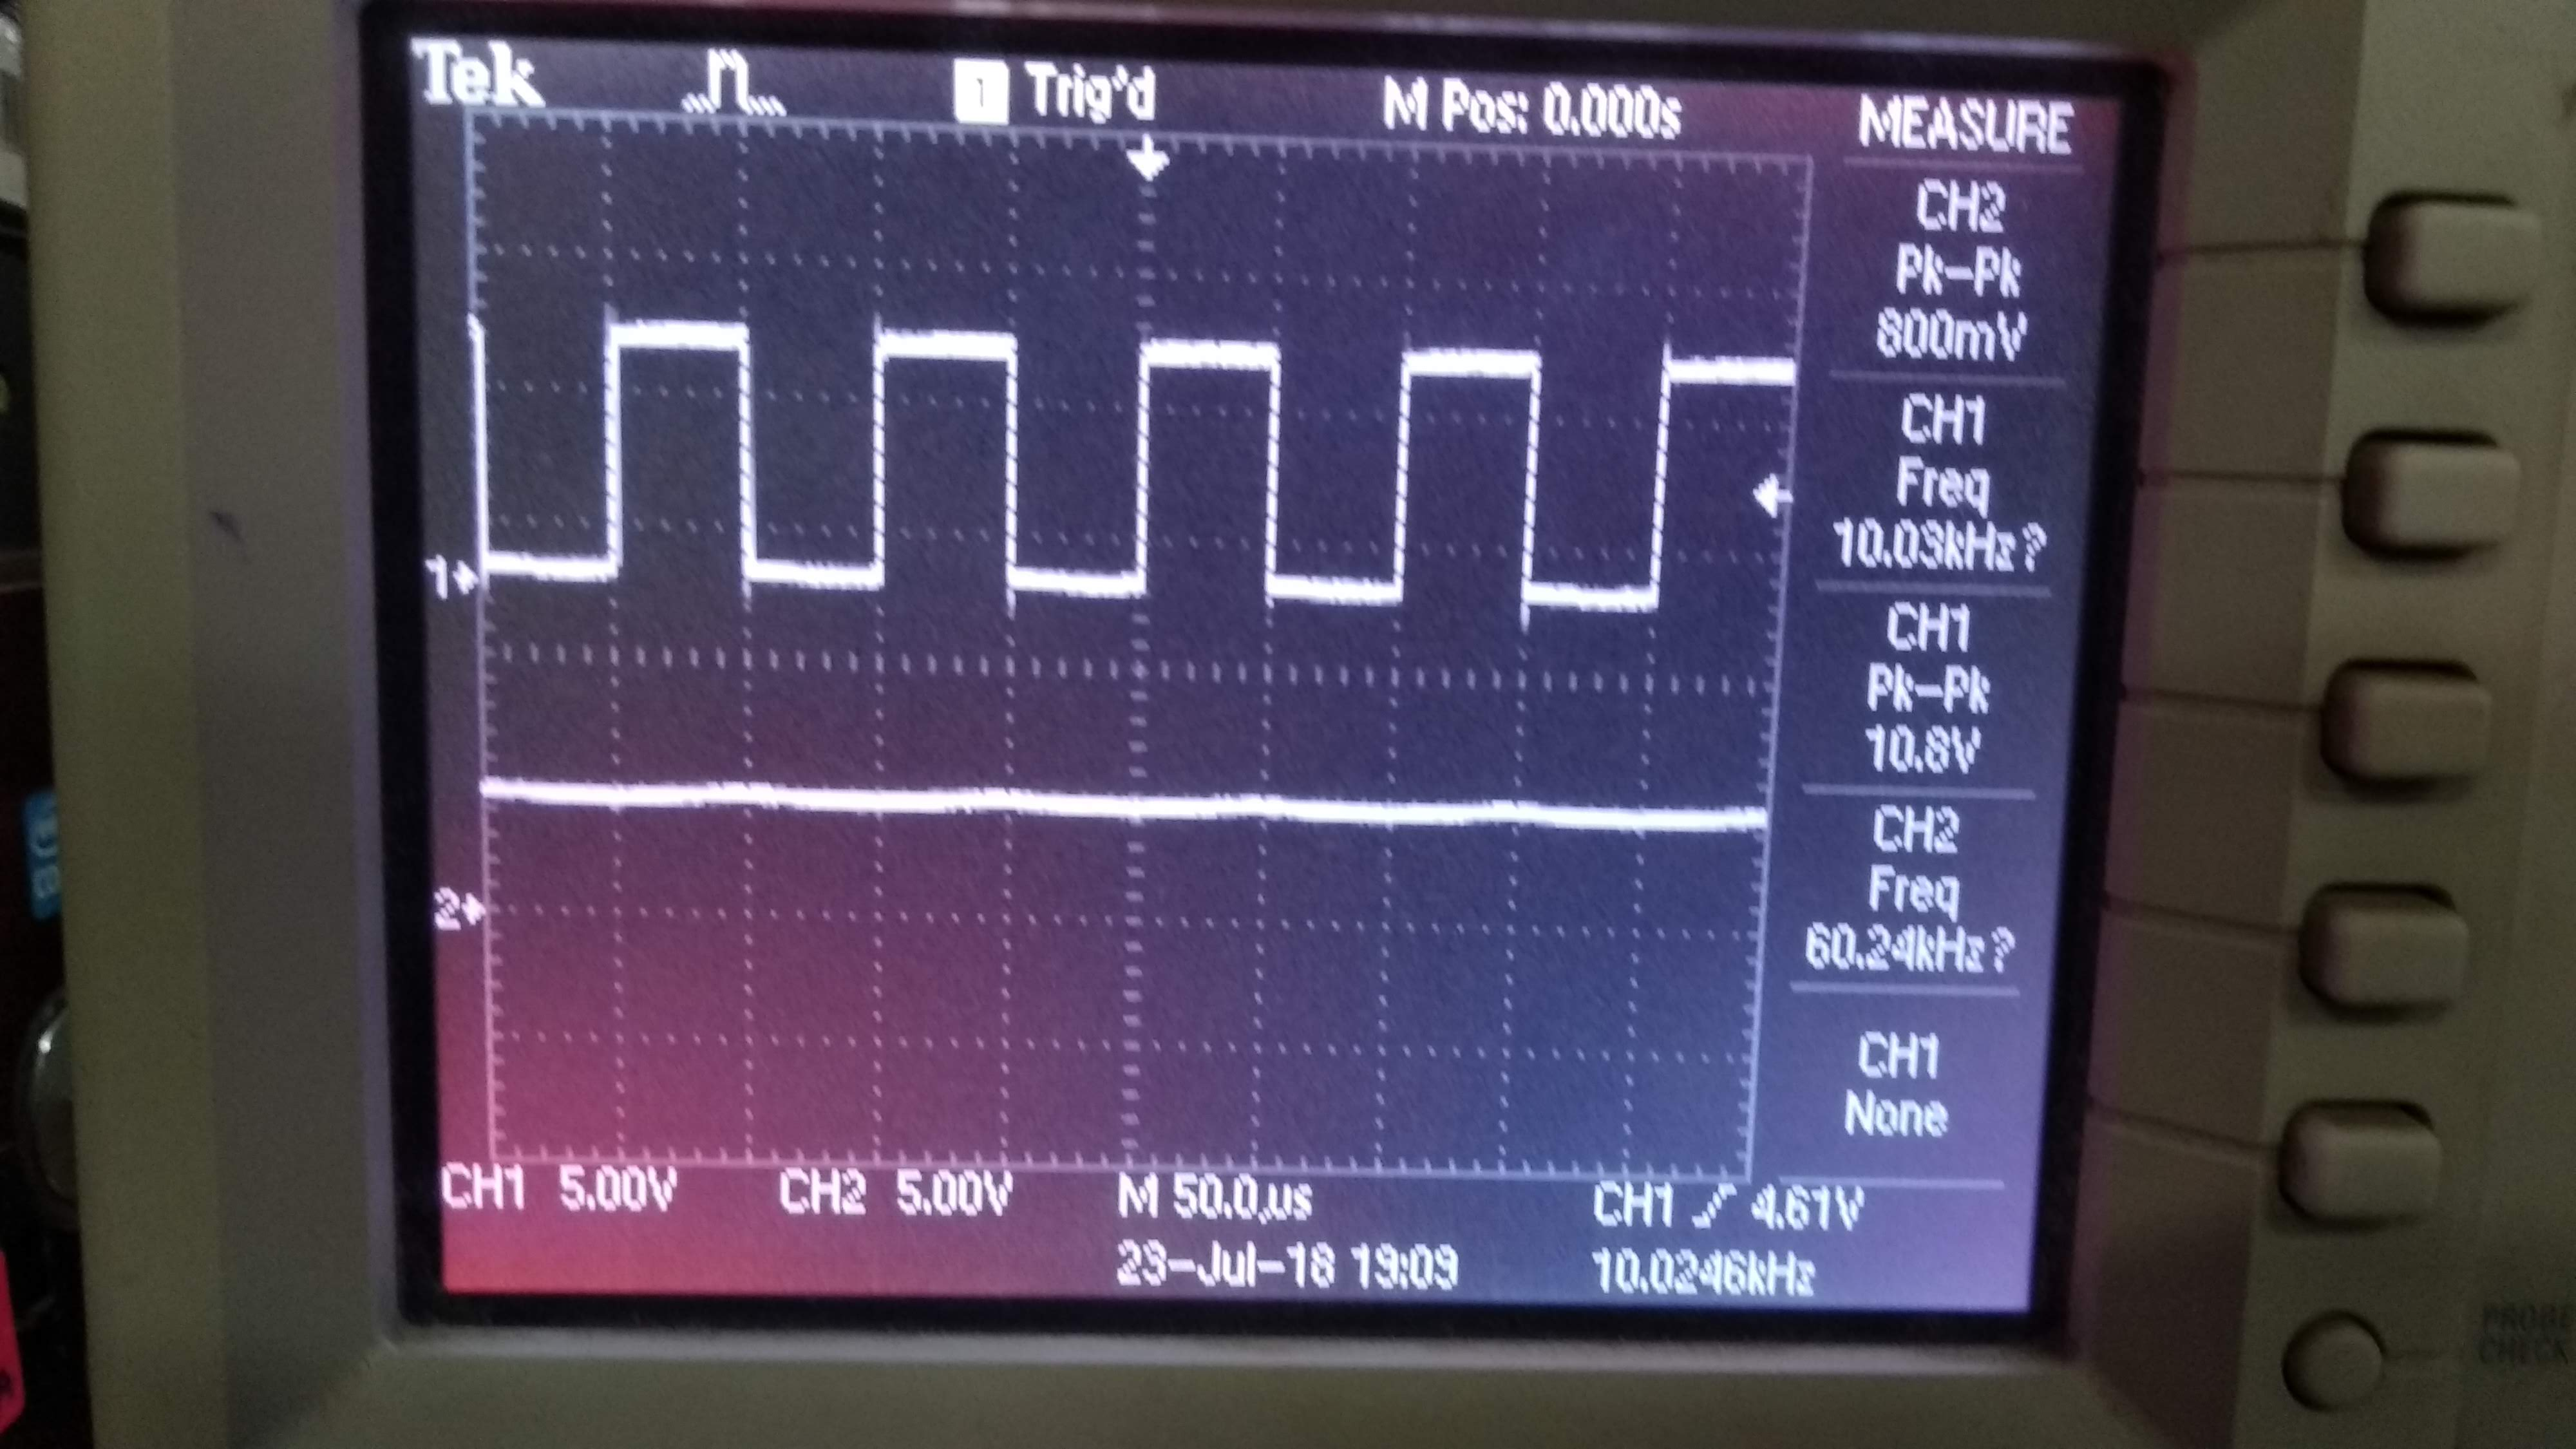
\includegraphics[scale = 0.08]{10khz.jpg}
\end{figure}

\begin{figure}
\centering
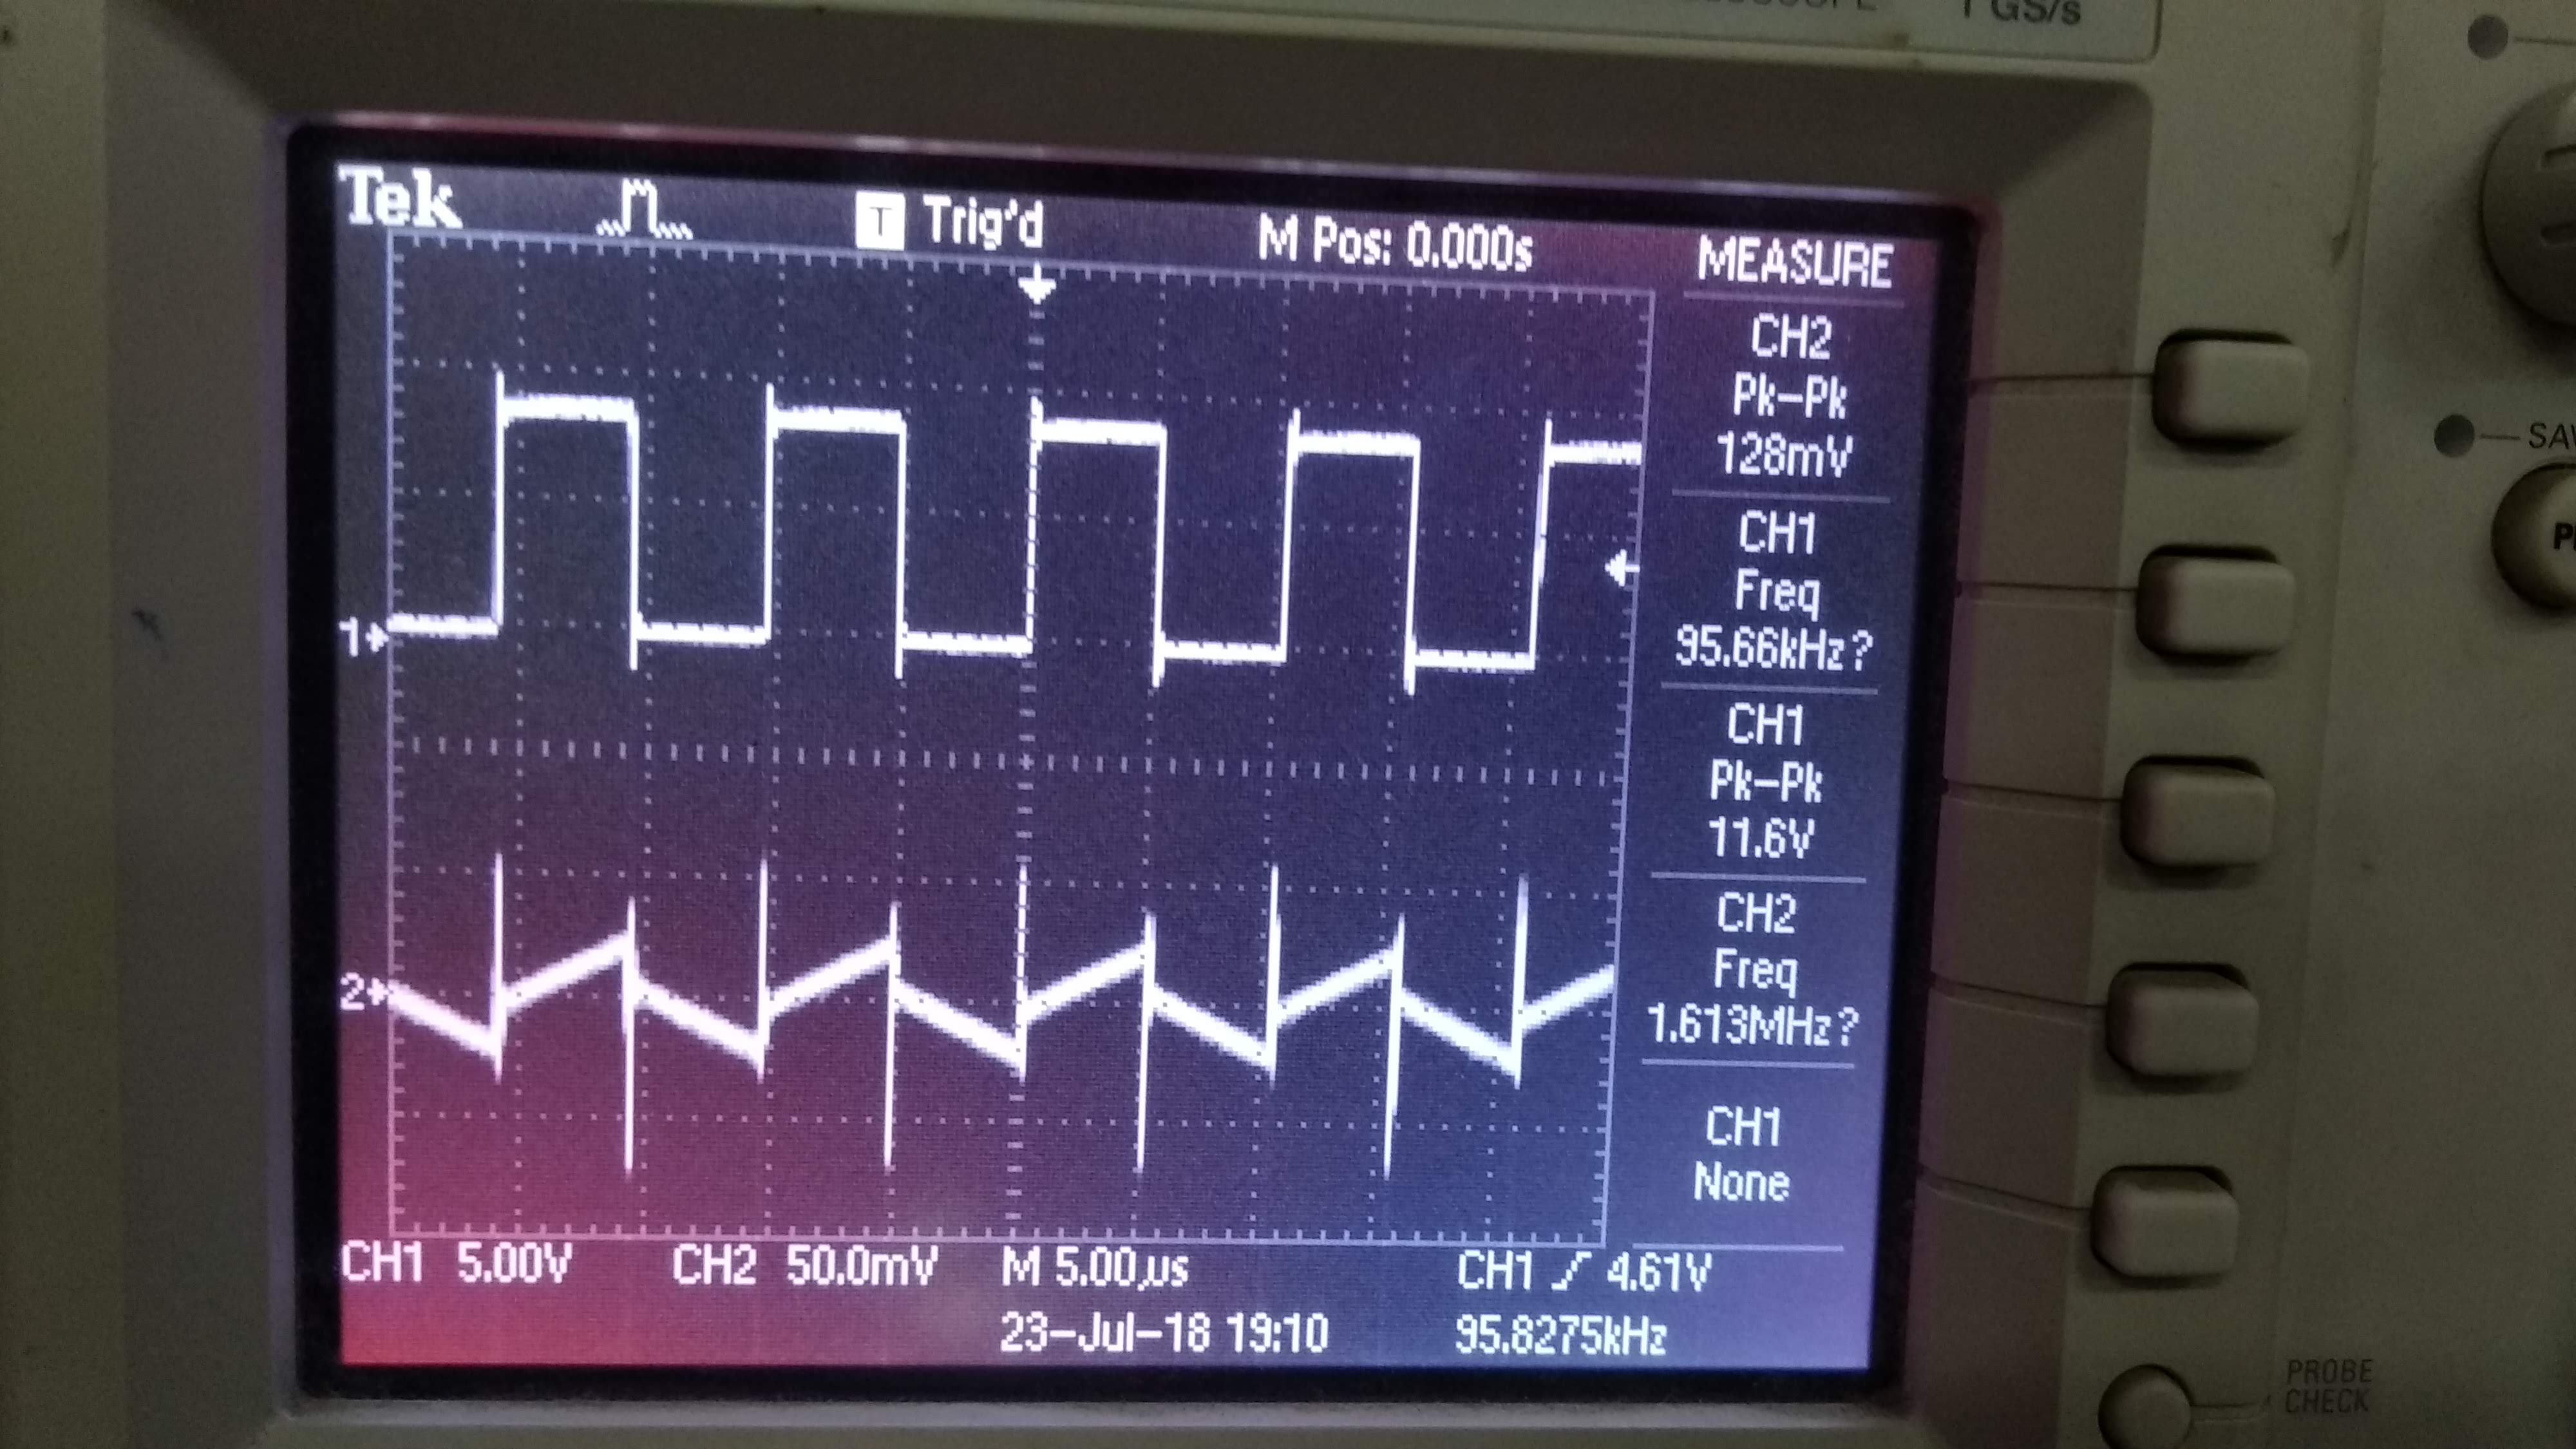
\includegraphics[scale = 0.08]{ac-coupling.jpg}
\end{figure}


\begin{figure}
\centering
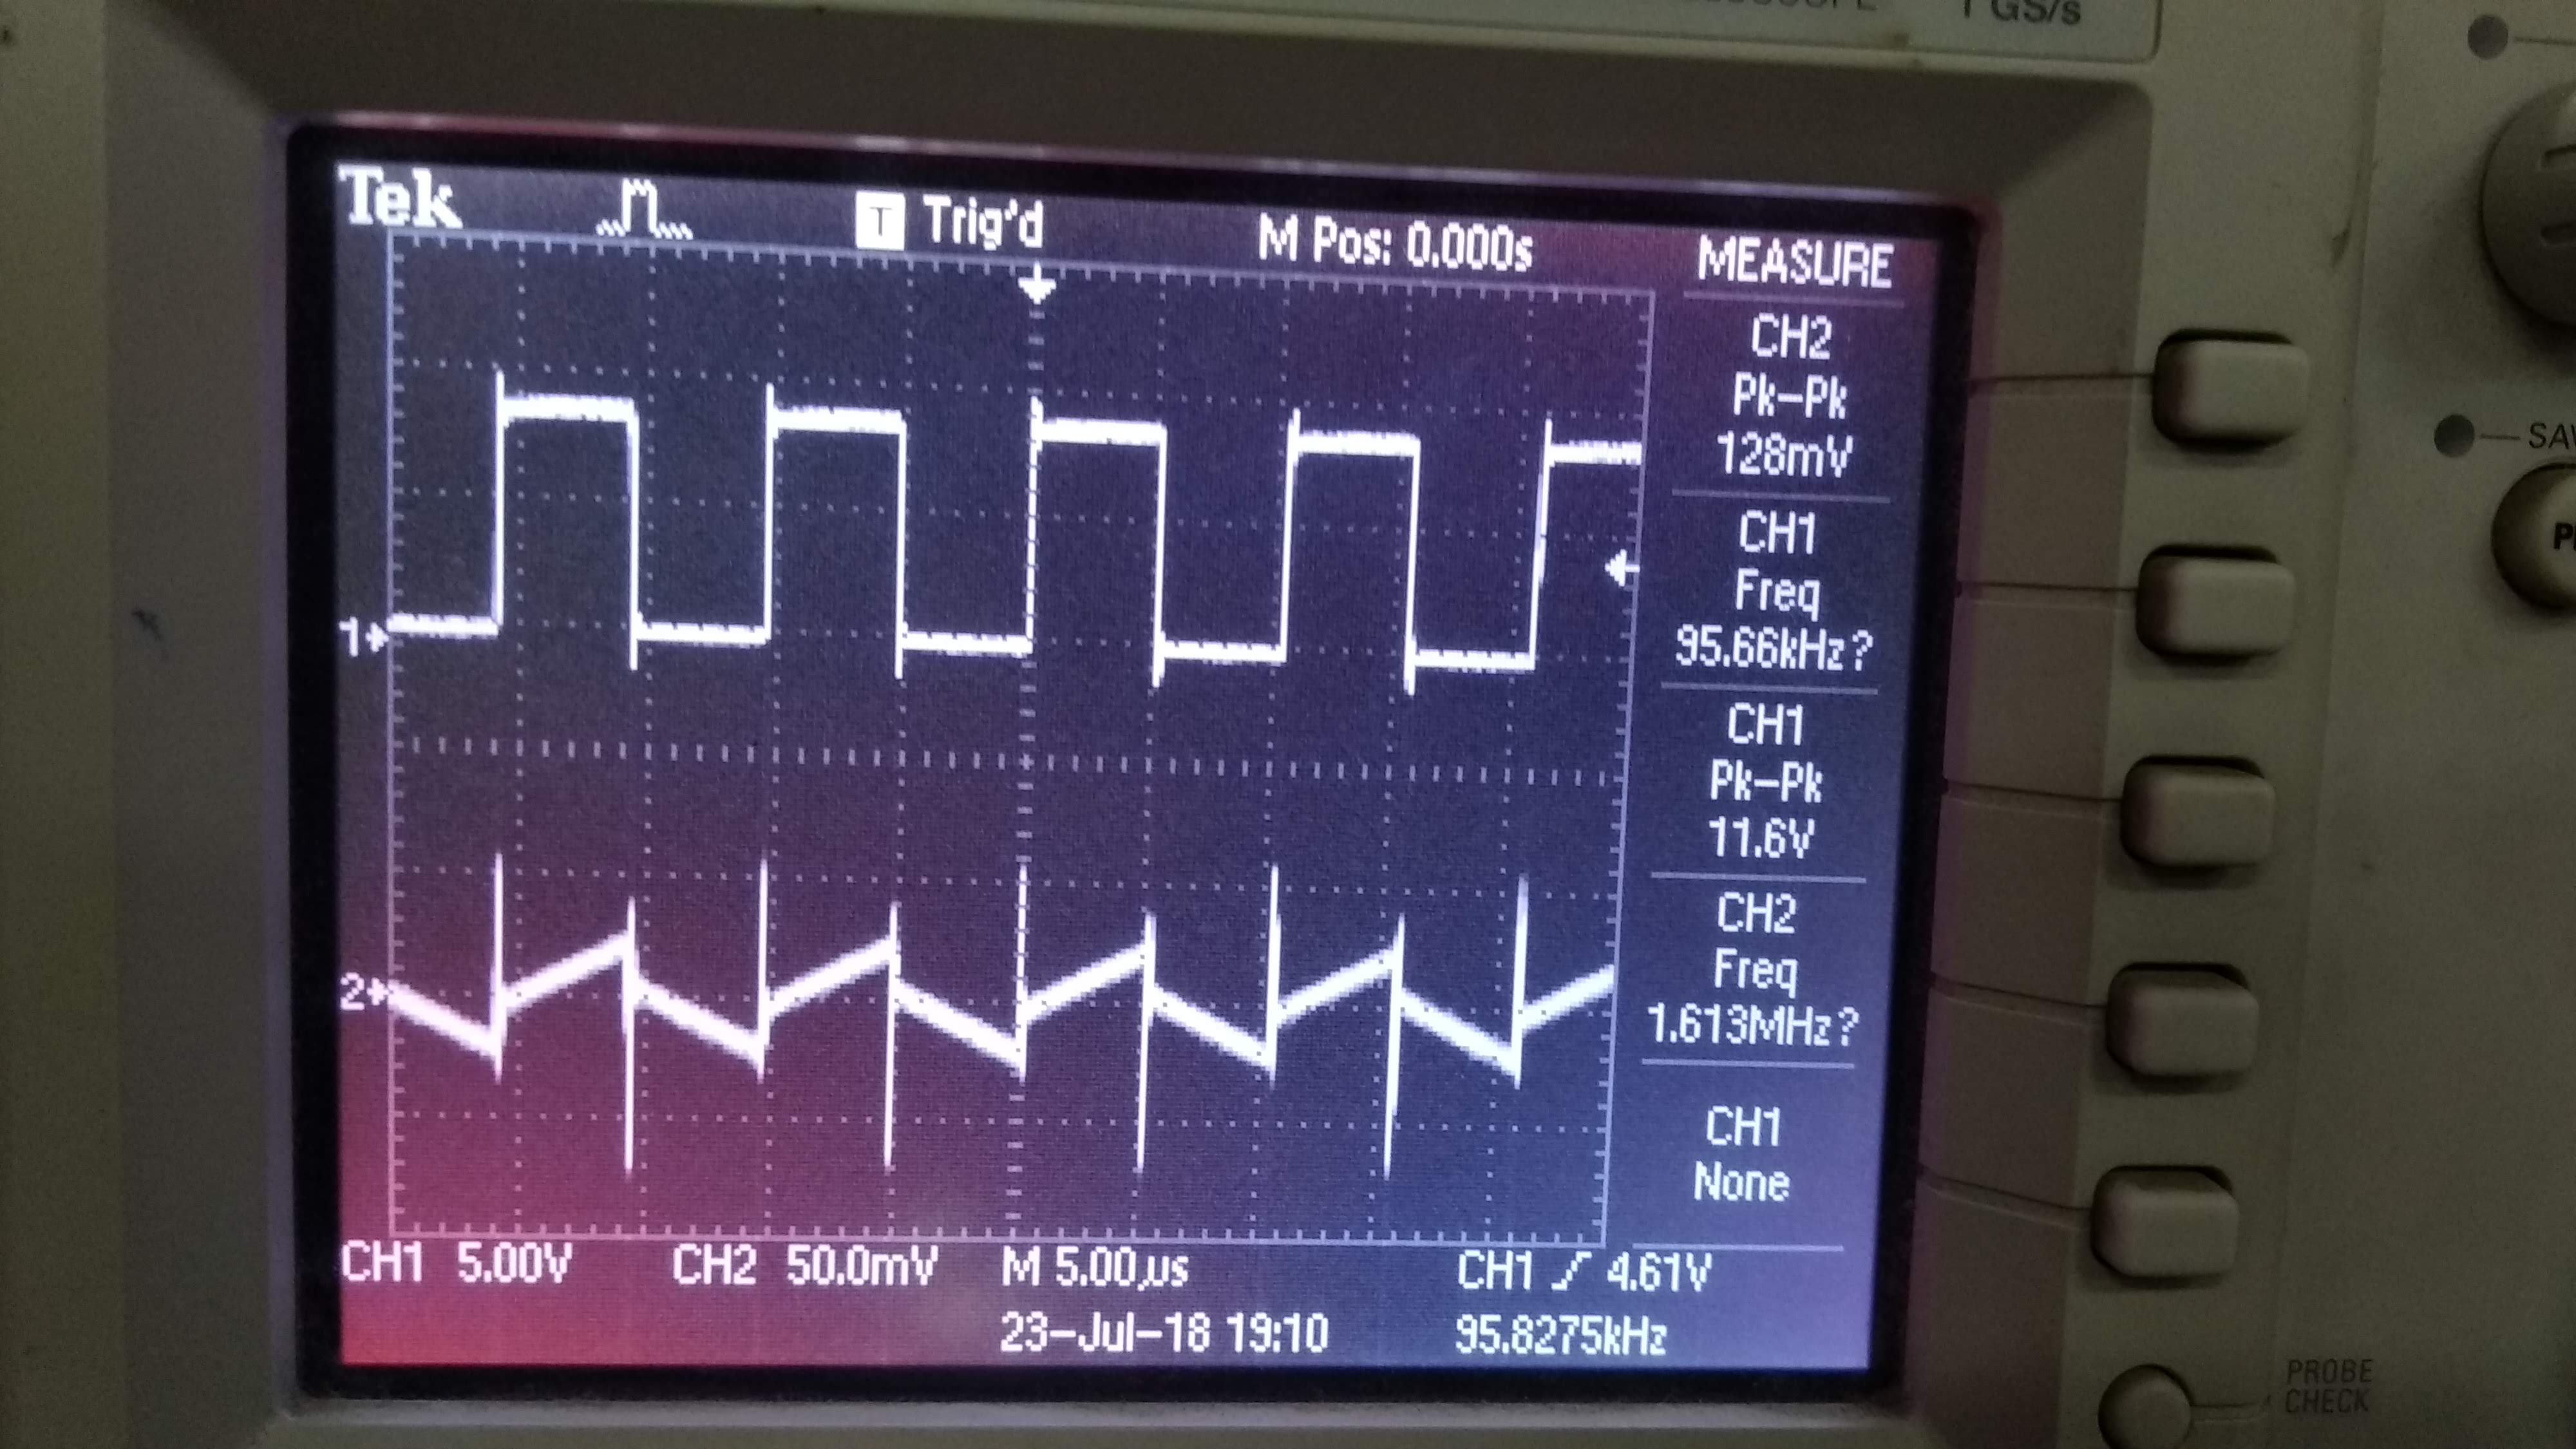
\includegraphics[scale = 0.08]{ac-coupling.jpg}
\end{figure}
\begin{figure}[h]
\centering



\end{figure}
\newpage
\subsection{Optional part }

Add your observations and comments on any additional(optional) exercises you perform


\section{Experiment completion status}
In this part , mention which sections you completed in lab and which you couldn't,also give suitable explanation stating why you couldn't complete it.

\section{Questions for reflection}
Address all the reflection questions here which will be given at end of each lab.
  

\end{document}
